\section{Code repositories}\label{code-repositories}

The complete implementation of AKF is available on GitHub at the
following locations:

\begin{itemize}
\tightlist
\item
  Core libraries (\passthrough{\lstinline!akflib!}):
  \url{https://github.com/lgactna/akflib}
\item
  The AKF agent for Windows (\passthrough{\lstinline!akf\_windows!}):
  \url{https://github.com/lgactna/akf-windows}
\item
  Standalone CASE/UCO 2.0 bindings for Python
  (\passthrough{\lstinline!caselib!}):
  \url{https://github.com/lgactna/CASE-pydantic}
\end{itemize}

The \passthrough{\lstinline!akf\_windows!} repository contains a sample
declarative script utilizing every implemented declarative module,
demonstrating nearly all existing AKF functionality. It also contains an
equivalent imperative script that was generated using
\passthrough{\lstinline!akf-translate!}. Both scripts, and some of their
outputs, can be found in the \passthrough{\lstinline!./scenarios!}
folder.

\section{Comparison of ForTrace and AKF
agents}\label{comparison-of-fortrace-and-akf-agents}

Invoking commands in ForTrace
\cite{gobelForTraceHolisticForensic2022} is straightforward; at the
network level, commands are performed by issuing a simple string to the
agent running on the target VM. For example, invoking a command to add a
new user to the VM can be seen in \autoref{lst:b.2.a}:

\begin{lstlisting}[label={lst:b.2.a}, caption={Creating a new user through ForTrace agent commands}, language=Python]
# From Demo.py
guest = virtual_machine_monitor1.create_guest(guest_name=imagename, platform="windows")

# Wait for the VM to connect to the VMM
guest.waitTillAgentIsConnected()
# create userManagement object
userManagement_obj = guest.application("userManagement", {})

# Add different users
logger.info("Adding user1")
try:
    userManagement_obj.addUser("user1", "password")
    while userManagement_obj.is_busy is True:
        time.sleep(1)
except Exception as e:
    print("An error occured: ")
    print(e)
time.sleep(5)
\end{lstlisting}

The agent's main loop, which receives and interprets these commands, is
also straightforward. A simplified version of the main loop is depicted
in \autoref{lst:b.2.b}:

\begin{lstlisting}[label={lst:b.2.b}, caption={Simplified ForTrace agent entry point}, language=Python]
def main():
    # create logger
    logger = create_logger('guestAgent', logging.INFO)

    logger.info("create Agent")
    a = Agent(operating_system=platform.system().lower(), logger=logger)
    logger.info("connect to fortrace controller: %s:%i" % (fortrace_CONTROLLER_IP, fortrace_CONTROLLER_PORT))
    a.connect(fortrace_CONTROLLER_IP, fortrace_CONTROLLER_PORT)

    # let all network interfaces come up
    time.sleep(15)

    # inform fortrace controller about network configuration
    a.register()

    # wait for commands
    while 1:
        time.sleep(1)
        a.receiveCommands()
\end{lstlisting}

When the \passthrough{\lstinline!Agent!} is instantiated, it binds a TCP
socket to the configured port and IP address, where it expects the
server (the VMM) to issue commands.
\passthrough{\lstinline!Agent.receiveCommands()!} executes commands by
reading the socket, parsing the received content, and then invoking
\passthrough{\lstinline!Agent.do\_command()!}, which converts the
command message into a specific Python function call with arguments.

The server, or ``virtual machine monitor'' (VMM), issues commands over
TCP to a running instance of the agent on the VM. Each module under
\passthrough{\lstinline!fortrace.application!} can be thought of as a
coherent group of commands associated with a particular user application
(such as Firefox or Thunderbird). Recall from \autoref{lst:b.2.a} how we
found our \passthrough{\lstinline!userManagement!} application and
invoked \passthrough{\lstinline!addUser!}; a simplified snippet is
depicted in \autoref{lst:b.2.c}:

\begin{lstlisting}[label={lst:b.2.c}, caption={Minimal ForTrace application API usage}, language=Python]
userManagement_obj = guest.application("userManagement", {})
userManagement_obj.addUser("user1", "password")
\end{lstlisting}

At a high level, the \passthrough{\lstinline!application()!} call
attempts to import
\passthrough{\lstinline!fortrace.application.\{application\_name\}!}.
Although not enforced by a higher-level interface, each of these modules
contains subclasses of the following four classes (defined in
\passthrough{\lstinline!fortrace.application.application!}) at minimum,
with additional helper classes for OS-specific functionality or other
modularity as needed:

\begin{itemize}
\tightlist
\item
  \passthrough{\lstinline!ApplicationVmmSide!}: Contains one function
  for each command implemented in
  \passthrough{\lstinline!ApplicationGuestSide!}. Each function builds a
  message that will be interpreted and acted upon by the corresponding
  \passthrough{\lstinline!ApplicationGuestSideCommands!} class.
\item
  \passthrough{\lstinline!ApplicationVmmSideCommands!}: Accepts and
  interprets module-specific messages returned by the agent, which may
  be used to update the remote state as tracked by the host.
\item
  \passthrough{\lstinline!ApplicationGuestSide!}: Implements the actual
  application-specific functionality for the agent, providing one
  function for each available command.
\item
  \passthrough{\lstinline!ApplicationGuestSideCommands!}: Interprets
  commands and arguments, calling the respective function in the
  corresponding \passthrough{\lstinline!ApplicationGuestSide!} subclass.
  This allows the actual dispatch of commands to be delegated to this
  class, which is free to choose how actions are performed (such as the
  use of threading and multiprocessing) as well as any module-wide state
  it may need to maintain.
\end{itemize}

This naming convention is intentional, as individual modules dictate the
name of the module in camelcase. For example,
\passthrough{\lstinline!fortrace.application.userManagement!} contains
\passthrough{\lstinline!UserManagementVmmSide!},
\passthrough{\lstinline!UserManagementVmmSideCommands!}, and so on.
Discovering and getting handles to these classes is performed through
string manipulation of the relevant application's module name, as shown
in \autoref{lst:b.2.d} (an abridged version of the
\passthrough{\lstinline!Agent.do\_command()!} method):

\begin{lstlisting}[label={lst:b.2.d}, caption={Demonstration of ForTrace agent module discovery and command execution}, language=Python]
def do_command(self, command):
    com = command.split(" ")
    package = com[0]
    module = com[1]

    # load class moduleGuestSide and moduleGuestSideCommands
    name = "fortrace." + package + "." + module
    self.logger.debug("module to load: " + name)
    mod = __import__(name, fromlist=[''])
    self.logger.debug("module '" + module + "' will be loaded via __import__")
    class_commands = getattr(mod, module[0].upper() + module[1:] + 'GuestSideCommands')
    
    class_commands.commands(self, app_obj, " ".join(com[1:]))
\end{lstlisting}

In the example above,
\passthrough{\lstinline!UserManagementGuestSide.addUser()!} contains the
code to execute on the guest when \passthrough{\lstinline!addUser()!} is
called, such as adding the registry keys needed for a user to be
created. On the other hand,
\passthrough{\lstinline!UserManagementVmmSide.addUser()!} contains the
code to send a message over TCP that the agent will understand,
eventually leading to the execution of the agent's version of
\passthrough{\lstinline!addUser()!}.

More precisely, the \passthrough{\lstinline!ApplicationVmmSide!}
subclass effectively serves as the API for calling the associated
functions in the \passthrough{\lstinline!ApplicationGuestSide!} class
running on the virtual machine. This subclass, along with the complete
agent-side code, is stored in a single file. For example, the API and
code for opening a Firefox browser window can be seen in
\autoref{lst:b.2.e}:

\begin{lstlisting}[label={lst:b.2.e}, caption={Sample ForTrace agent API implementation}, language=Python]
class WebBrowserFirefoxVmmSide(ApplicationVmmSide):
    def open(self, url):
        """Sends a command to open a webBrowserFirefox on the associated guest.

        @param url: Website to open.
        """
        try:
            self.logger.info("function: WebBrowserFirefoxVmmSide::open")
            self.url = url
            self.window_id = self.guest_obj.current_window_id
            self.guest_obj.send(
                "application " + "webBrowserFirefox " + str(self.window_id) + " open " + self.webBrowserFirefox + " " + self.url)

            self.guest_obj.current_window_id += 1
        except Exception as e:
            raise Exception("error WebBrowserFirefoxVmmSide::open: " + str(e))

# Example usage:
browser = WebBrowserFirefoxVmmSide()
browser.open("google.com")
\end{lstlisting}

Calling the \passthrough{\lstinline!open()!} command from the host sends
a structured message to the agent, generally of the form seen in
\autoref{lst:b.2.f}:

\begin{lstlisting}[label={lst:b.2.f}, caption={Sample ForTrace agent protocol message}, ]
application webBrowserFirefox <window id> open Firefox <url>
\end{lstlisting}

Upon receiving this message, the agent's main loop will search for the
\passthrough{\lstinline!webBrowserFirefox!} module and import its
corresponding \passthrough{\lstinline!ApplicationGuestSideCommands!}
subclass. After any state management, the subclass will then search for
a function called \passthrough{\lstinline!open!} in its corresponding
\passthrough{\lstinline!ApplicationGuestSide!} class, as implemented in
\autoref{lst:b.2.g}:

\begin{lstlisting}[label={lst:b.2.g}, caption={Corresponding ForTrace agent-side call }, language=Python]
class WebBrowserFirefoxGuestSide(ApplicationGuestSide):
    def open(self, args):
        # docstring omitted
        try:
            arguments = args.split(" ")
            web_browser = arguments[0]
            url = arguments[1]

            if len(arguments) > 2:
                self.timeout = arguments[2]
            else:
                self.timeout = 30

            self.logger.info(self.module_name + "GuestSide::open")
            self.last_driven_url = url
            self.logger.debug("URL to call: " + url)

            self.logger.info("open url: " + url)

            self.helper.run_firefox()  # start ff session

            retval = self.helper.navigate_to_url(url)  # browse to the specified url
            if not retval:
                self.logger.warning("could not open url")

            self.agent_object.send("application " + self.module_name + " " + str(self.window_id) + " opened")

            self.agent_object.send("application " + self.module_name + " " + str(self.window_id) + " ready")
            self.window_is_crushed = False
        except Exception as e:
            # Some logging/teardown...
            self.window_is_crushed = True
            self.agent_object.send("application " + self.module_name + " " + str(self.window_id) + " error")
\end{lstlisting}

As described in \autoref{the-akf-agent}, this is achieved in AKF using RPyC services, which are analogous
to the \passthrough{\lstinline!ApplicationGuestSideCommands!} and
\passthrough{\lstinline!ApplicationGuestSide!} classes of individual
ForTrace modules. In addition to providing the RPyC services themselves,
agents also implement an API to call these services using typed
functions.

For example, suppose we wanted to implement functionality similar to the
ForTrace code above, allowing users to navigate to a webpage. An
equivalent RPyC service and its corresponding API may be implemented as
seen in \autoref{lst:b.2.h}:

\begin{lstlisting}[label={lst:b.2.h}, caption={Minimal reimplementation of ForTrace module as an RPyC service}, language=Python]
# Server-side code
class ChromiumService(AKFService):
    def exposed_set_browser(
        self, browser_type: Literal["msedge", "chrome"], profile: str = "Default"
    ) -> BrowserContext:
        # Various setup code...
        self.browser = chromium.launch_persistent_context(
            headless=False,
            user_data_dir=profile_path,
            channel=browser_type,
            args=[f"--profile-directory={profile}"],
        )

        return self.browser

# Client-side API
class ChromiumServiceAPI(WindowsServiceAPI):
    def __init__(self, host: str, port: int) -> None:
        """
        Initialize the API with an RPyC connection to the service.
        """
        self.rpyc_conn = rpyc.connect(
            host,
            port,
            config={"sync_request_timeout": None},
        )

    def set_browser(
        self, browser_type: Literal["msedge", "chrome"], profile: str = "Default"
    ) -> BrowserContext:
        self.browser = self.rpyc_conn.root.set_browser(browser_type, profile)
        return self.browser
\end{lstlisting}

Implementing support for a particular service on the client-side API is
as simple as calling an untyped function
\passthrough{\lstinline!rpyc\_conn.root.set\_browser()!}. By wrapping it
around a typed function,
\passthrough{\lstinline!ChromiumServiceAPI.set\_browser()!}, users
regain the ability to use code completion and static linting tools.

\section{CASE Python bindings}\label{case-python-bindings}

As described in \autoref{case-and-python-bindings}, CASE is defined using Turtle, allowing objects to be
written in a human-readable text format. For example, the following set
of triples in \autoref{lst:b.3.a} describes an object called
\passthrough{\lstinline!ApplicationFacet!} with two properties,
\passthrough{\lstinline!numberOfLaunches!} and
\passthrough{\lstinline!applicationIdentifier!}:

\begin{lstlisting}[label={lst:b.3.a}, caption={Example CASE object definition for applications \cite{UcoProjectUCO2025}}, ]
observable:ApplicationFacet
    a
        owl:Class ,
        sh:NodeShape
        ;
    rdfs:subClassOf core:Facet ;
    rdfs:label "ApplicationFacet"@en ;
    rdfs:comment "An application facet is a grouping of characteristics unique to a particular software program designed for end users."@en ;
    sh:property
        [
            sh:datatype xsd:integer ;
            sh:maxCount "1"^^xsd:integer ;
            sh:nodeKind sh:Literal ;
            sh:path observable:numberOfLaunches ;
        ] ,
        [
            sh:datatype xsd:string ;
            sh:maxCount "1"^^xsd:integer ;
            sh:nodeKind sh:Literal ;
            sh:path observable:applicationIdentifier ;
        ] ,
        ...
        ;
    sh:targetClass observable:ApplicationFacet ;
    .
\end{lstlisting}

An instance of an \passthrough{\lstinline!Application!} object may thus
be represented in the JSON-LD format using the
\passthrough{\lstinline!ApplicationFacet!} as seen in
\autoref{lst:b.3.b}, including some attributes omitted from the example
in \autoref{lst:b.3.a}:

\begin{lstlisting}[label={lst:b.3.b}, caption={Instantiated CASE application object as JSON-LD }, ]
{
    "@id": "kb:dcec8d09-a8bc-4b7c-93ab-16c7b363d48b",
    "@type": "uco-observable:Application",
    "uco-core:hasFacet": [
        {
            "@id": "kb:68004de9-1139-405f-aea7-2c05f3a84709",
            "@type": "uco-observable:ApplicationFacet",
            "uco-observable:numberOfLaunches": 12,
            "uco-observable:applicationIdentifier": "test"
        },
    ]
}
\end{lstlisting}

The CASE project provides official Python bindings
\cite{CaseworkCASEMappingPython}. One notable implementation detail
is that it stores all object attributes in a dictionary after
instantiation. This can be seen in the example of an
\passthrough{\lstinline!ApplicationFacet!} in \autoref{lst:b.3.c} below.
Intuitive usage suggests that the
\passthrough{\lstinline!application\_identifier!} attribute is
accessible through the \passthrough{\lstinline!facet!} object, but it
must instead be accessed as a dictionary key with a non-intuitive name.

\begin{lstlisting}[label={lst:b.3.c}, caption={Sample usage of official CASE Python bindings \cite{CaseworkCASEMappingPython}}, language=Python]
facet = ApplicationFacet(application_identifier = "test", number_of_launches=3)

# These attributes do not exist
facet.application_identifier
facet.number_of_launches

# The number of launches must be accessed as a dictionary key, which
# does not return a simple integer; instead, it returns a
# dictionary
app_facet['uco-observable:numberOfLaunches']
# -> {"@type": "xsd:integer", "@value": "3"}
\end{lstlisting}

AKF's Pydantic-based bindings greatly simplify the declaration of
individual CASE objects while allowing typical attribute-based access.
For example, AKF's complete declaration of
\passthrough{\lstinline!ApplicationFacet!} is shown in
\autoref{lst:b.3.d}:

\begin{lstlisting}[label={lst:b.3.d}, caption={Example of Pydantic-based CASE object declaration used by AKF}, language=Python]
from typing import Optional

from uco import core

# ... Other object definitions in same file

class ApplicationFacet(core.Facet):
    installedVersionHistory: ApplicationVersion | list[ApplicationVersion] | None = []
    operatingSystem: ObservableObject | None = Field(
        default=None, json_schema_extra={"IRI": True}
    )
    numberOfLaunches: int | None = None
    applicationIdentifier: str | None = None
    version: str | None = None
\end{lstlisting}

This definition is only eight lines, which is 27 lines shorter than the
declaration of \passthrough{\lstinline!ApplicationFacet!} provided by
the CASE project's existing Python bindings (excluding the docstring).

A simple CASE bundle, representing the complete contents of a forensic
scenario, can be constructed and exported to JSON-LD using AKF libraries
as shown in \autoref{lst:b.3.e}:

\begin{lstlisting}[label={lst:b.3.e}, caption={Demonstration of bundle serialization using the AKF Python bindings for CASE}, language=Python]
from caselib import case, uco

bundle = uco.core.Bundle(
    description="An Example Case File",
    specVersion="UCO/CASE 2.0",
    tag="Sample artifacts",
)

url_object = uco.observable.ObservableObject()
url_facet = uco.observable.URLFacet(fullValue="www.docker.com/howto")
url_object.hasFacet.append(url_facet)
bundle.object.append(url_object)

with open("example.jsonld", "wt+") as f:
    data = bundle.model_dump(serialize_as_any=True)
    f.write(json.dumps(data, indent=2))
\end{lstlisting}

Although the UCO/CASE 2.0 Python bindings developed as part of AKF
significantly improve usability and flexibility over the existing CASE
bindings, several limitations of the library do not make it fully
compliant with the CASE ontology. In particular, the Python bindings aim
to keep object definitions as simple as possible, preferring native
Python types where possible. This means that some information from the
ontology is lost when converting them to their respective Python class.
Several examples include:

\begin{itemize}
\tightlist
\item
  \textbf{Datatypes}: Many XSD datatypes are not equivalent between the
  turtle files and Python bindings. For example, the arbitrary-precision
  \passthrough{\lstinline!xsd:decimal!} type is represented as a native
  Python float, but is also written out as a native JSON float on
  serialization to JSON-LD. The resulting datatype is
  \passthrough{\lstinline!xsd:float!}, which may cause information to be
  lost.
\item
  \textbf{Vocabularies}: Many CASE ``vocabularies'', a datatype in which
  a field's value should be chosen from a fixed set of values, are
  correctly converted to native Python string enumerations. However, the
  vocabulary datatype is not serialized, only the value; thus, the
  resulting JSON-LD makes no indication that the selected value is
  actually from the vocabulary datatype, even if the value itself is
  inside the vocabulary set. For example, if the string ``MD5'' is a
  member of the \passthrough{\lstinline!HashNameVocab!} datatype, our
  Python bindings serialize this as a standard
  \passthrough{\lstinline!xsd:string!}, not
  \passthrough{\lstinline!vocabulary:HashNameVocab!}.
\item
  \textbf{Field names}: Some fields of CASE objects, such as the
  \passthrough{\lstinline!from!} field of an email message, are reserved
  Python keywords that may not be used as the name of a variable. To
  solve this, we append an underscore to any fields that would violate
  this rule when automatically generating Pydantic classes from the
  Turtle RDF files. However, the original name of the field is not
  preserved when serializing objects; although the simplest fix is to
  remove trailing underscores when serializing, a more robust solution
  may be to attach the ``original'' name to the Pydantic field.
\item
  \textbf{Dangling references}: There are no built-in mechanisms to
  ensure that an object is serialized in its ``full'' form at least
  once; that is, a user could place references to an object identifier
  throughout the document without adding the object being referred to.
\end{itemize}

Additionally, one major feature of CASE/UCO is not currently supported.
CASE allows objects to be of multiple types at once, such as a disk
image marked as both an \passthrough{\lstinline!observable:File!} and an
\passthrough{\lstinline!observable:Image!}. Python types can inherit
from multiple types, but a single object may not be multiple types at
once; it might be necessary to create a ``wrapper'' type that
encompasses both types and correctly serializes these types as expected.

\section{Historical declarative
syntaxes}\label{historical-declarative-syntaxes}

While designing the declarative syntax for AKF, the syntaxes of D-FET
\cite{williamCloudbasedDigitalForensics2011}, SFX
\cite{russellForensicImageDescription2012}, and Yannikos et al.
\cite{yannikosDataCorporaDigital2014} were reviewed. For
completeness, brief examples of scenarios in each of these synthesizers
are included here. Notably, none of these works provide details on how
the parser of their declarative languages is implemented. Similarly, few
details are provided about the architecture and design of the code used
to carry out actions based on interpreted declarative instructions. This
lack of detail may be attributed to the fact that the scenario creation
enabled by these declarative syntaxes, rather than the syntaxes
themselves, was the primary focus of these works.

\textbf{D-FET} \cite{williamCloudbasedDigitalForensics2011} uses a
custom language that does not depend on any existing text-based
languages, as seen in the simple scenario in \autoref{lst:b.4.a}:

\begin{lstlisting}[label={lst:b.4.a}, caption={Sample D-FET declarative scenario without events \cite{williamCloudbasedDigitalForensics2011}}, ]
INSTANCE LOAD [Image=WINDOWS2003] 
MOUNT INSTANCE [Disk=STANDARDDISK] AS [Partition="c"] 
ACTIVITY LOAD [Number=12] [Type=JPEG IMAGES; Class=DRUGS] 
    INTO [Folder=USER FOLDER] 
    AT [Period=1 MINUTE] [Interval=INTERVAL] 
    FOR [User=Fred]
\end{lstlisting}

The scenario above will create an instance based on the WINDOWS2003
image from the Host Forensics Image library (which contains pre-created
images from OS installation discs). It will then load 12 JPEG images
from the ``DRUGS'' class of images using the ``STANDARDDISK'' disk
image. This appears to create a host with \emph{predefined}, but not
\emph{timed} activity -- the machine simply begins in this state rather
than simulating a user doing this over some period of time.

To generate timed activity that can be placed on a timeline, D-FET
allows users to add ``events.'' The sequence of events in
\autoref{lst:b.4.b} directs the synthesizer to log in as a user, delete
files, and log out.

\begin{lstlisting}[label={lst:b.4.b}, caption={Extension of the D-FET declarative scenario with events \cite{williamCloudbasedDigitalForensics2011}}, ]
INSTANCE LOAD [Image=WINDOWS2003] 
MOUNT INSTANCE [Disk=STANDARDDISK] AS [Partition="c"] 
ACTIVITY LOAD [Number=12] [Type=JPEG IMAGES; Class=DRUGS] 
    INTO [Folder=USER FOLDER] 
    AT [Period=1 MINUTE] [Interval=INTERVAL] 
    FOR [User=Fred]
ACTIVITY EVENT [Event=LOGIN; User=Fred] 
ACTIVITY EVENT [Event=DELETEFILE; User=Fred; File=JPEF IMAGES] 
ACTIVITY EVENT [Event=LOGOUT; User=Fred ]
\end{lstlisting}

\textbf{SFX} \cite{russellForensicImageDescription2012} uses an
XML-based language with tags and attributes that are easily readable ,
as shown in \autoref{lst:b.4.c}:

\begin{lstlisting}[label={lst:b.4.c}, caption={Sample SFX declarative scenario expressed as XML \cite{russellForensicImageDescription2012}}, language=XML]
<disk size="512M" alignment="cylinder" diskid="0x12345678">
    <partition index="p1" hidden="0" size="48M" type="vfat">
        <expand archive="part1.zip" />
        <copy from="fake.dat" to="/fake01.dat" />
        <copy from="fake.dat" to="/fake02.dat" />
        <delete from="/Thomas.jpg" />
    </partition>
    <partition index="p2" hidden="0" size="48M" type="ntfs">
        <base os="windows7x64" />
        <copy from="fake.dat" to="/fake03.dat" />
        <copy from="fake.dat" to="/fake04.dat" />
        <user username="Gordon">
            <browserhistory browser="firefox">
                <url link="[http://bbc.co.uk"](http://bbc.co.uk") time="13:14:00 1 Jan 2013" />
            </browserhistory>
        </user>
    </partition>
    <partition index="p3" hidden="1" size="64M" type="ntfs">
        <expand archive="part3.zip" />
        <copy from="fake.dat" to="/fake11.dat" />
        <copy from="fake.dat" to="/fake12.dat" />
        <delete from="/docs/image.exe" />
        <slackspace offset="20" file="/tomas.gif" message="This is a secret message" />
    </partition>
    <partition index="s1" hidden="0" size="144M" type="ext3">
        <base os="fedora15x64" />
        <expand archive="part2.tar" />
        <copy from="fake.dat" to="/tmp/fake01.dat" />
        <copy from="fake.dat" to="/tmp/fake02.dat" />
    </partition>
</disk>
\end{lstlisting}

Here, a user can define multiple partitions on a single disk, each with
a distinct filesystem that may or may not contain an underlying
operating system. SFX allows users to generate artifacts in multiple
ways, with each unique application- or OS-specific feature using a
distinct XML element name. Artifact generation features include copying
files to the guest machine in bulk, inserting files in the slack space
of an existing file, and using browser artifacts.

Finally, the work of Yannikos et al.
\cite{yannikosDataCorporaDigital2014} is particularly notable
because it appears to be fully GUI-based, expecting users to visually
construct Markov chains to define scenarios. An example scenario from
their publication can be seen in Figure \autoref{fig:yannikos-gui}:

\begin{figure}[h]
\centering
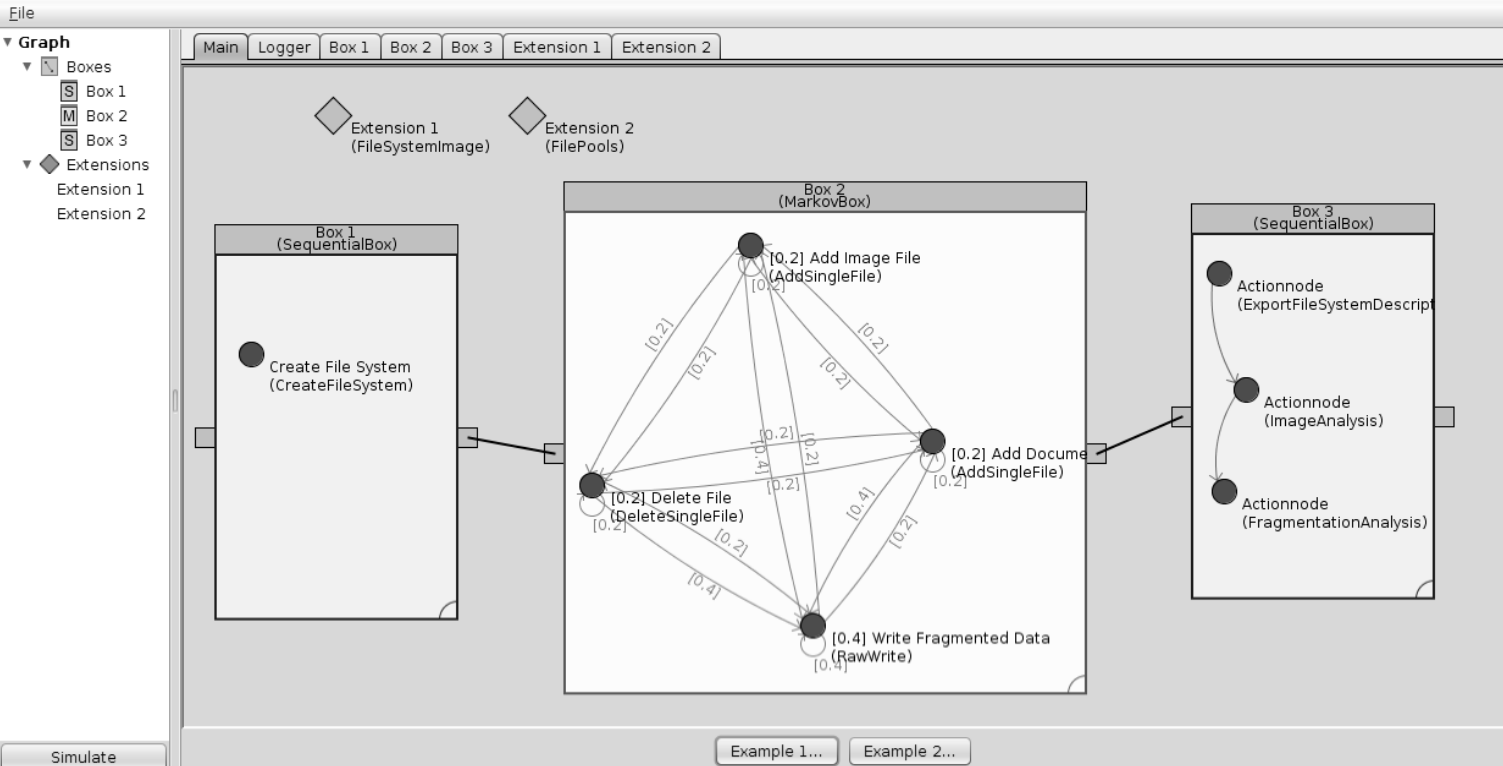
\includegraphics[width=1\linewidth]{yannikos.png}
\caption{GUI-based scenario declaration from Yannikos et al.
\cite{yannikosDataCorporaDigital2014}}\label{fig:yannikos-gui}
\end{figure}

Although details are relatively limited, each node appears to be a
distinct action that can be automated. Individual nodes accept
parameters that can be used to configure how their associated artifacts
are created. Each ``box'' encompasses a complete Markov chain, with
transitions from one box to another occurring after an unknown condition
is fulfilled. Finally, the diamonds outside the boxes, known as
extensions, are libraries that provide extra functionality during the
execution of the overall scenario.
